\chapter{Testbeam}
Studying the properties of sensor modules is crucial for an optimal performance of particle detectors. The new pixel modules used for the ATLAS ITk upgrade have to be thoroughly
tested in terms of efficiency and radiation hardness to fulfill the necessary requirements for their installment.
In order to evaluate the sensor's performance they are irradiated in testbeam experiments similar to the conditions in the LHC.
These beam test measurements are performed mainly in two testbeam facilities, being located at Cern and Deutsches Elektronen Synchrotron (DESY). Sensors that are planned to be
installed in the ATLAS ITk are tested at DESY during the LS2.

\section{DESY Testbeam}
DESY is a national research center located in Hamburg. It operates the electron synchrotron DESY II since 1987 initially to accelerate electrons before injecting them into
HERA, the largest synchrotron at DESY. After the shut down of HERA in 2007, DESY II is now used for testbeam measurements. It produces an electron beam with energies up to
$\SI{7}{\GeV}$, which collides with a carbon fiber target creating bremsstrahlung in the process. The photons are extracted and collide with a secondary target
converting them to electron-positron pairs. A dipole magnet behind the target creates a homogenous magnetic field to filter out unwanted energies and particles. This process
is shown schematically in figure \ref{fig:testbeam}.

\begin{figure}
  \centering
  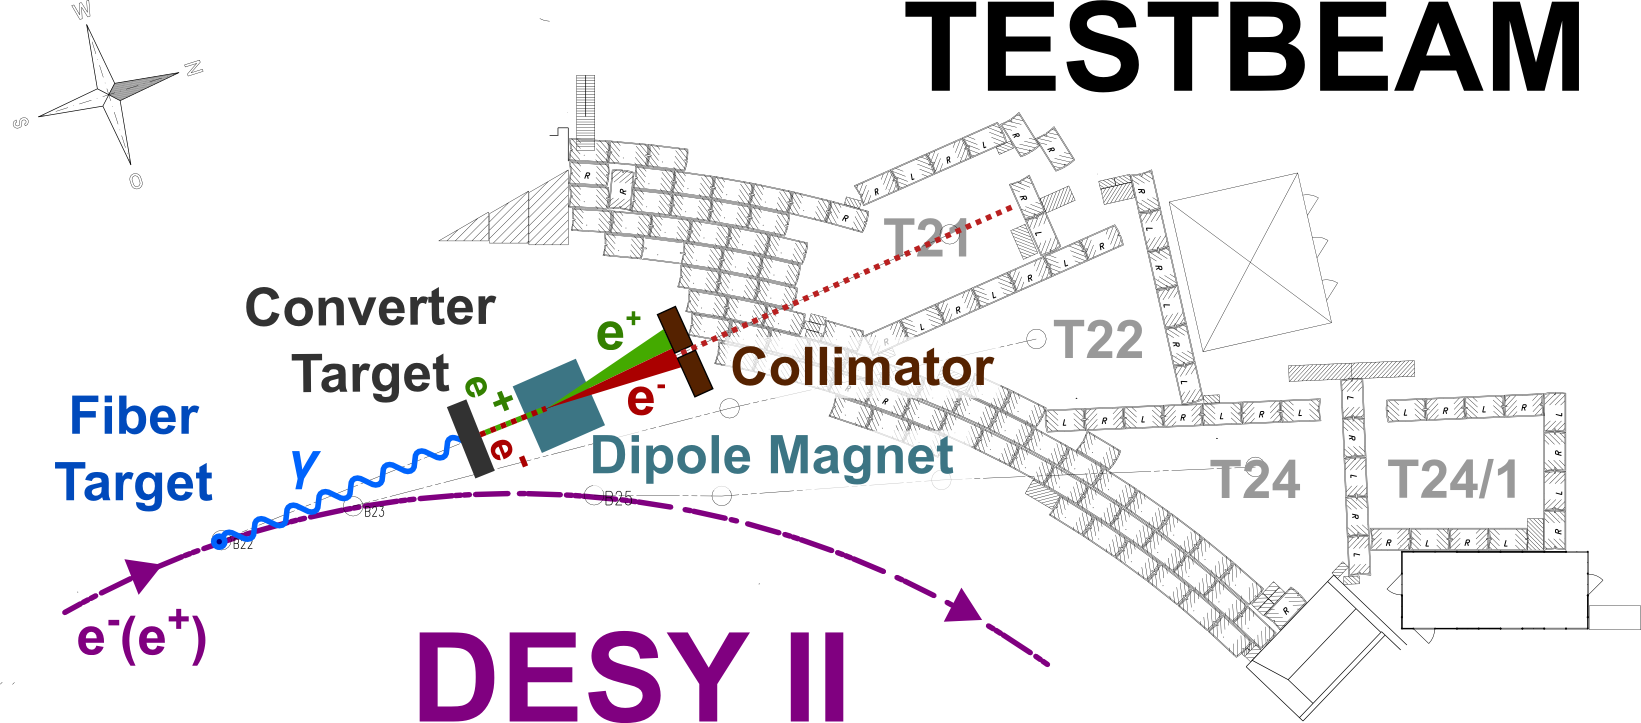
\includegraphics[height=0.4\textwidth]{images/desy.png}
  \caption{Depiction of the beam generation in testbeam experiments going through the beam line TB21 \cite{testbeam}.}
  \label{fig:testbeam}
\end{figure}

The permanently installed EUDET-type Pixel Beam telescopes DATURA and DURANTA are located behind the beamlines TB21 and TB22 and enable the tracking of the particles
produced by DESY II. Both telescopes consist of six Mimosa26 monolithic active pixel sensors with %a pixel pitch of $\SI{18.4}{\micro\meter} \times \SI{18.4}{\micro\meter}$.
three sensors each incorporated into one arm of the telescope and the DUT's being placed in between. A polystyrene box filled with dry ice is used to cool the DUT's to
avoid annealing and other unwanted effects due to heat. For time references during the measurements, an FE-I4 sensor is placed behind the telescope with a
time resolution of $\SI{25}{\nano\second}$ The sensors contain $336 \times 80$ pixels with a
$\SI{50}{\micro\meter} \times \SI{250}{\micro\meter}$ pixel pitch. Figure \ref{fig:telescope} shows the telescope setup of DATURA.

%\begin{figure}
%  \centering
%  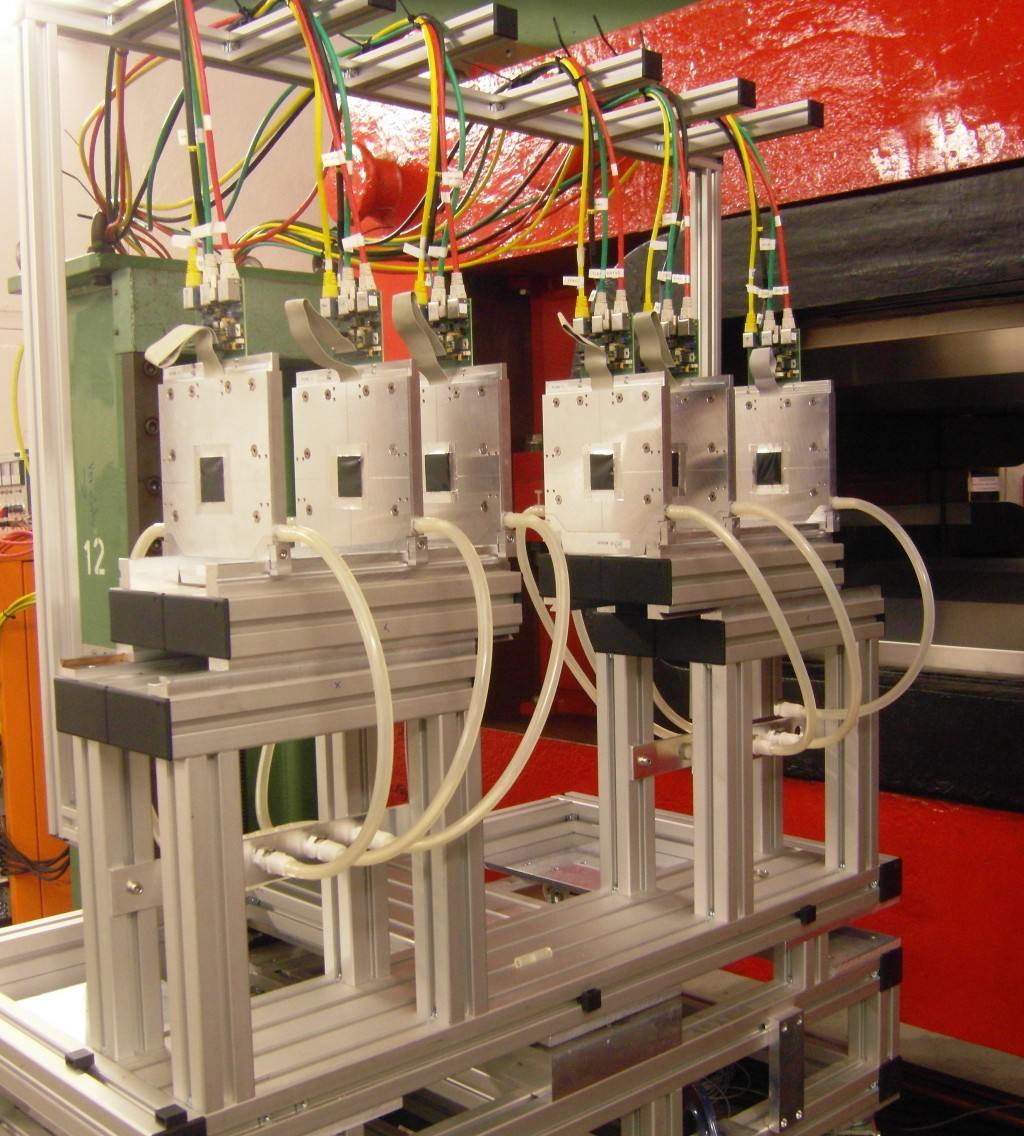
\includegraphics[height=0.4\textwidth]{images/telescope.jpg}
%  \caption{Shown is the Beam telescope DATURA consisting of six Mimosa26 sensors placed in the jigs. The tubes connected to the sensors transport water to
%  cool the sensors \cite{telescope}.}
%  \label{fig:telescope}
%\end{figure}

\begin{figure}
  %\centering
  \begin{subfigure}{0.48\textwidth}
      \centering
      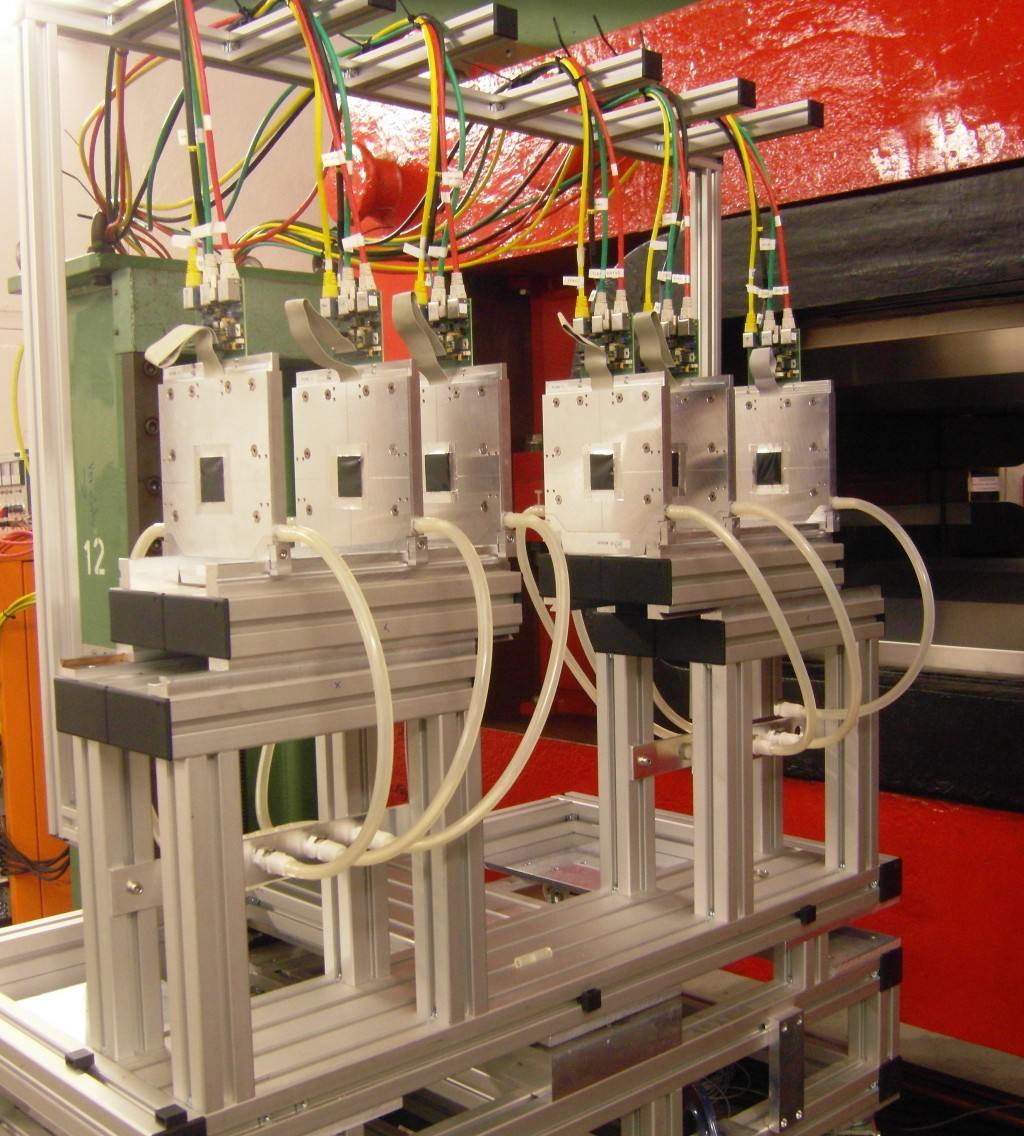
\includegraphics[height=0.82\textwidth]{images/telescope.jpg}
  \end{subfigure}
  \begin{subfigure}{0.48\textwidth}
      %\centering
      \hspace{-1cm}
      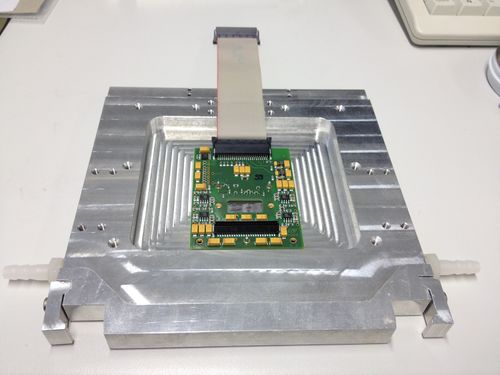
\includegraphics[height=0.82\textwidth]{images/mimosa.jpg}
  \end{subfigure}
  \caption{Shown on the left is the Beam telescope DATURA consisting of six Mimosa26 sensors placed in the jigs. The tubes connected to the sensors transport water to
  cool the sensors \cite{telescope}. Shown on the right is the Mimosa26 board inside the aluminium housing \cite{mimosa}. }
  \label{fig:telescope}
\end{figure}

The Mimosa26 sensors are fabricated in a standard $\SI{0.35}{\micro\meter}$ CMOS process with a fast binary read-out
%size of $\SI{13.7}{\milli\meter} \times \SI{21.5}{\milli\meter}$.
Signals are measured with a time resolution of $\SI{230}{\micro\second}$ with each measurement in a read-out cycle belonging to the same event.
They contain $576 \times 1152$ pixels with a pixel pitch of $\SI{18.4}{\micro\meter} \times \SI{18.4}{\micro\meter}$
and a thickness of $\SI{50}{\micro\meter}$.

The generic data acquisition framework EUDAQ records the data produced in testbeam experiments. It centrally handles the data flow and synchronises data stream to enable
the integration of different independent devices under test. An exemplary setup of a beam telescope with EUDAQ is shown in figure \ref{fig:eudaq_bild}.
More information in \cite{eudaq}.

\begin{figure}
  \centering
  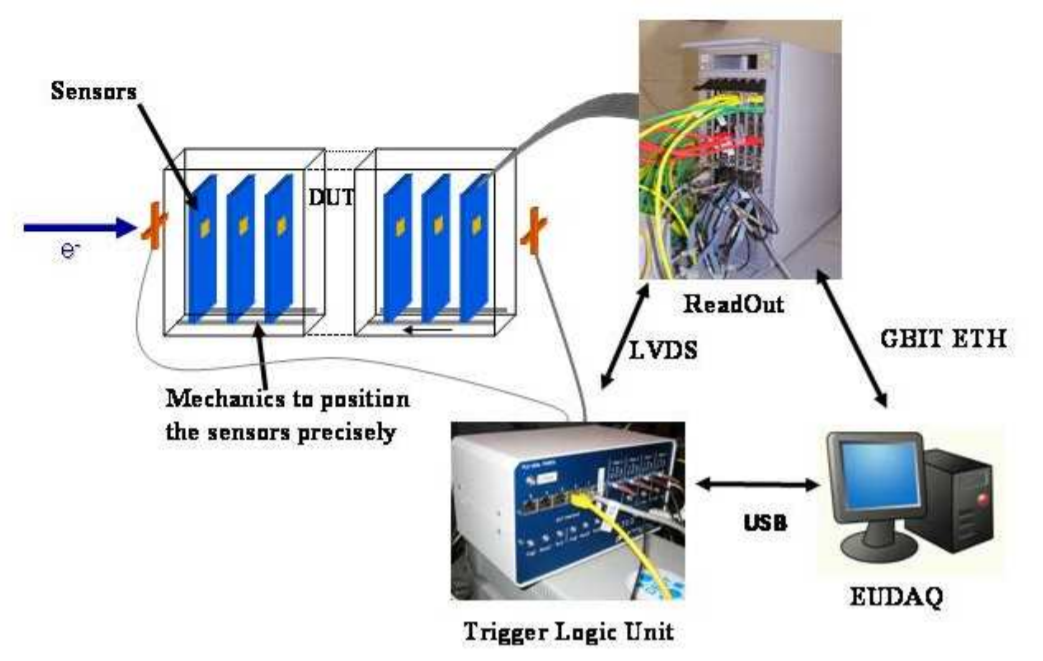
\includegraphics[height=0.4\textwidth]{images/eudaq.png}
  \caption{Necessary components for an analogue telescope \cite{eudaq_bild}.}
  \label{fig:eudaq_bild}
\end{figure}

\chapter{Track reconstruction}
The hit information of the sensor planes can be used to reconstruct the initial particle track. To properly reconstruct the tracks, multiple steps have to
be performed. For that reason, entire frameworks were created to allow for a versatile and accurate track reconstruction to be possible. Two of the most
developed reconstruction software were used in this thesis and are explained in the following.

\section{The track reconstruction framework EUTelescope}
In order to do that the software EUTelescope was developed and
primarily used since 2007. It uses the Modular Analysis and Reconstruction for the Linear Collider (MARLIN) framework, which is part of the
International Collider Software package (ILCSoft). Each step in the reconstruction depends on MARLIN processors, which read in data, modifies and outputs new data to be
taken by the next processors. The individual steps in the reconstruction will call on certain processors specified for its task resulting in a
modular structure.

Information about the telescope geometry is stored in  Geometry API for Reconstruction (GEAR) files. This includes the position and rotation
of the sensors as well as their pixel layouts. Further parameters like radiation hardness, magnetic field, and general properties of the used sensors have to be
specified to ensure proper track reconstruction.

General parameters and parameters in individual reconstruction steps are specified in the configuration file. This includes the import of the raw data and the
geometry file, the applied reconstruction steps, and the definition of the cuts. \\
The steering files define the processors used in each reconstruction step and in which order they are executed.
A complete track reconstruction with EUTelescope contains the converter, the clustering, the hitmaker, the alignment and the track fitting in this respective order.
The overall track reconstruction of EUTelescope is shown in figure \ref{fig:track_reco} with the most important steps explained in the following.

\begin{figure}
  \centering
  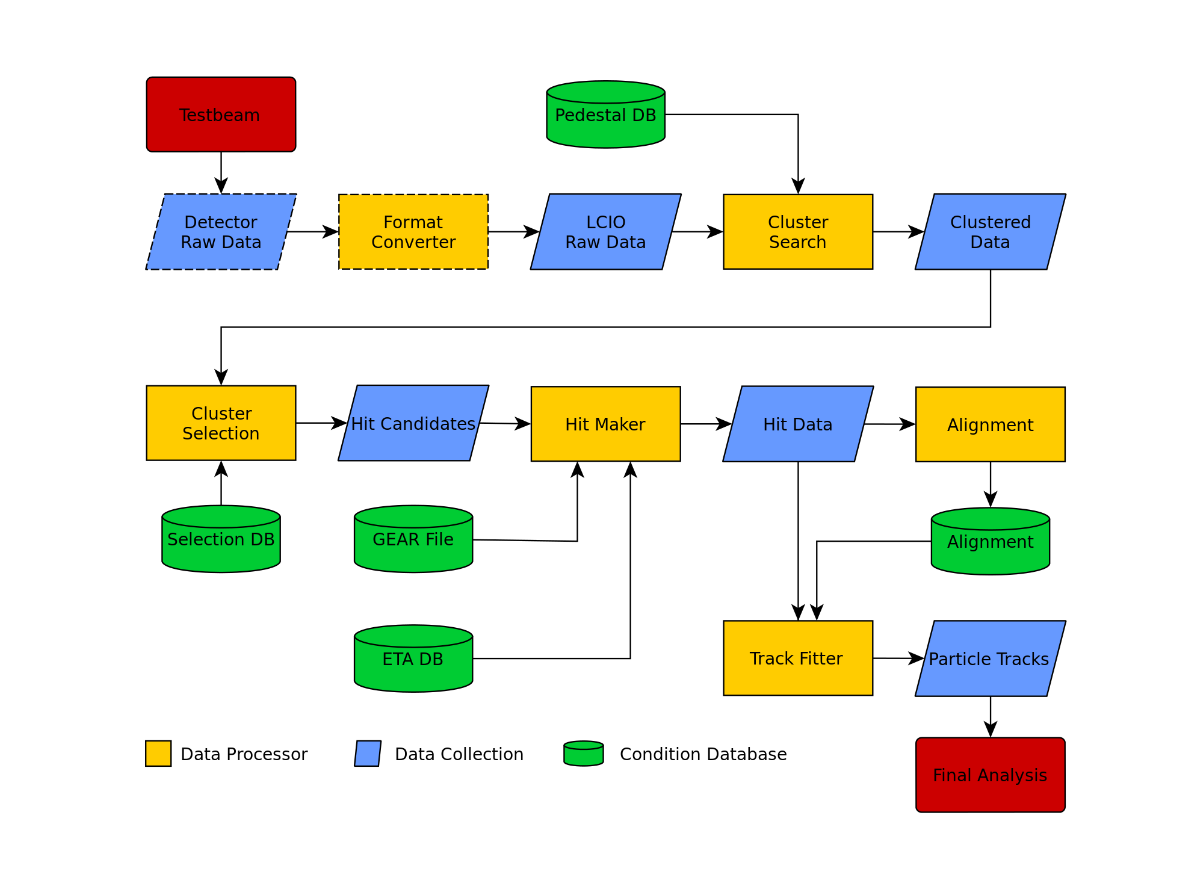
\includegraphics[height=0.6\textwidth]{images/track_reco.png}
  \caption{The overall track reconstruction of EUTelescope including the MARLIN processors and files. \cite{track_reco}.}
  \label{fig:track_reco}
\end{figure}

First, the raw data has to be converted to the lcio format for subsequent MARLIN processors. In addition, the module detects noisy pixels by analysing the
hit rate of the pixels and dividing them by the sum of measured events. The resulting firing frequency can be limited by user defined cuts, thus removing entries
from noisy pixels in the lcio file.

In the clustering process, hit information on a sensor plane generated by the same particle will be clustered. Clusters with more than one pixel occur due to
particles traversing through multiple pixels or charge sharing. Pixels will be grouped together based on their distance.
Regulation of the clustering process is then possible with cuts on the pixel distances.

The hitmaker step determines the particle's hit position, the cluster center, of each cluster. For one pixel cluster, the cluster center is equal to the middle of
the pixel. Cluster centers of clusters with more than one pixel are calculated with a charge-weighted center-of-gravity algorithm. This means, that
the deposited charge of each pixel is taken into account to derive the particle's position. The cluster centers are transformed to the global coordinate
system of the telescope to function as the hit position for the track reconstruction. Global hit information on the sensors of particle tracks is assumed to be correlated with only
a small spread of the beam angle, which makes an initial guess of the telescope alignment, the prealignment, possible. With the prealignment it is possible
to correct larger misplacements of the sensors.

To compensate for possible misalignment of sensors in the telescope, the alignment processor tries to optimise the setup. Cluster information from the hitmaker
is used to fit tracks through the planes and correct deviations by rotating and shifting the sensors. After the alignment process is finished a new gear file is produced, which
is then used for further reconstruction steps. Usually, several iterations of the alignment process occur to determine the optimal positions of the sensor planes
in the telescope.
There are two major processors for the alignment step, which implement different track fitting algorithms.
The DAF processor is based on a Kalman filter and was specifically designed for high noise environments. It uses the inbuild combinatorics filter, which fits
straight-line tracks through all combinations of clusters allowed by the specified cuts and only keeps the ones with a minimum $\chi^2$. Here, the $\chi^2$ parameter
describes the goodness of the fit and is defined as:
\begin{align} \label{eqn:chi}
  \chi^2 = \sum_i (r_x/\sigma_x)^2 + (r_y/\sigma_y)^2
\end{align}

The parameters $r_x$ and $r_y$ refer to the residuals on each sensor in the x- and y-direction, which describe the distance of the cluster center used for the track fit and the
position of the track on a plane. All residuals are weighted with their spatial resolution $\sigma_x$ and $\sigma_y$ for each sensor. \\
The second fitter uses the General Broken Line (GBL) algorithm with a separate pattern recognition processor for track fitting. Kinematics of
beam particles are used to predict hits belonging to a track. In the track finding process, two straight lines are fitted through the upstream and
downstream sensors, whenever the user-defined cuts on the slope allow it. The two straight lines are extrapolated to the centre of the telescope, where
they form the overall track depending on their distance to each other and the corresponding user-defined cut.\\
Fitted tracks used for the alignment are handled by the Millipede II processor. It performs least squares minimisation for a particular set of problems, which
have an interest in global parameters over local parameters in common. Thus, Millepede II is able to align the planes with any applied track model.

After the alignment is finished the tracks are fully reconstructed with either the DAF or the GBL fitter. Optionally, DUT's can be included in the fitting
process, however, it is usually avoided to keep the residuals of the DUT unbiased. In the scope of this thesis, the GBL processor is used for the
alignment and fitting step. To reconstruct a track, the fitGBL processor uses GBL points, which carry a series of attributes. These points can either be a
hit or another point of interest on the trajectory. Figure \ref{fig:gbl} depicts an exemplary reconstructed track with the fitGBL processor.

\begin{figure}
  \centering
  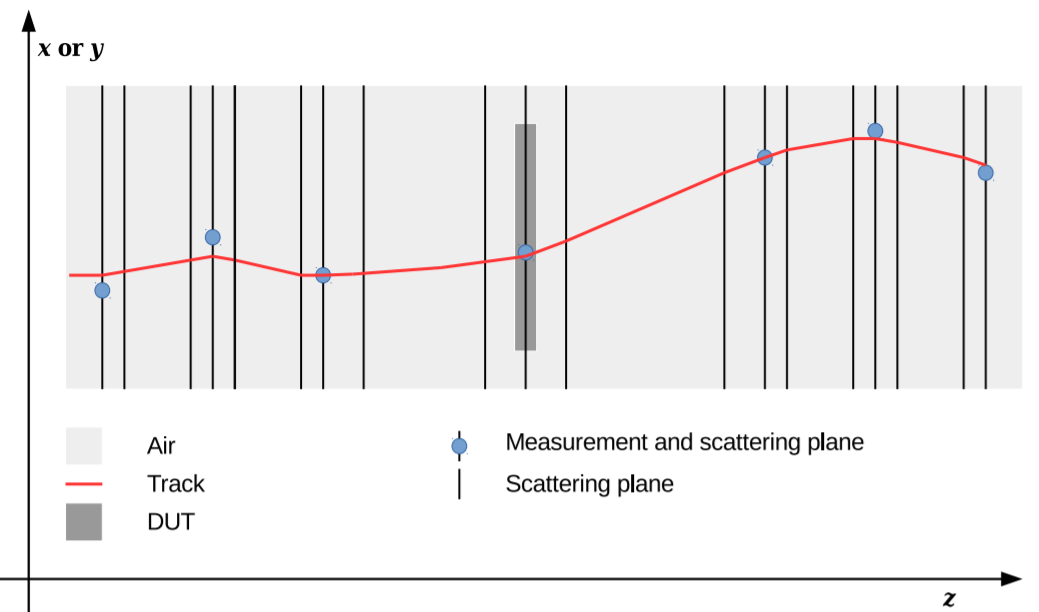
\includegraphics[height=0.5\textwidth]{images/gbl.png}
  \caption{Track reconstruction with the fitGBL processor. Scattering points are connected with a straight line. \cite{gbl}.}
  \label{fig:gbl}
\end{figure}



\section{The track reconstruction framework Corryvreckan}
Corryvreckan is a fast and lightweight track reconstruction framework released in 2017 and is the most developed alternative to the EUTelescope software.
Since the development and support of the EUTelescope discontinued, Corryvreckan is planned to supersede the former as the primarily used track
reconstruction software. Its main advantage is the minimal amount of external dependencies connected to the software and the more user-friendly usage of
it.
Corryvreckans structure is based on the modular concept of the simulation software Allpix$^2$, making the software flexible and ensures to meet the requirements for track reconstruction in
complex environments. Global parameters and modules used for the track reconstruction are specified in the configuration file, which starts the event loop upon
executing. Data and the geometry of the setup are both imported into the configuration file as well. A reference sensor has to be specified in the geometry folder
for which the rest of the telescope is aligned with.

During event processing, information taken and produced by the modules are temporarily stored on the clipboard, serving as the infrastructure for temporary
storing information. %the event, the
%temporary data storage and the persistent storage. The event is the central element storing information about the currently processed data.
The necessary steps in the track reconstruction chain of the software are similar to ones taken in EUTelescope and are explained in the following.

To load the taken data into Corryvreckan a certain eventloader module is used depending on the data format. The order of eventloader modules
is important as the first module loaded will define the event on the clipboard either through trigger numbers or a time window. Measurements stored with EUDAQ are loaded with the
EventloaderEUDAQ module, which requires the EUDAQ library as an external dependency. Alternatively to the eventloader modules, data in root format can also be imported
with the FileReader module, which is mainly used for simulated data or data written out with the FileWriter module.

The clustering process can be either done with the Clustering4D or the ClusteringSpatial module, with the former being the standard clustering module taking hit timestamps
into account. Spatial and timing cuts can be defined by the user either through absolute values or relative factors multiplied by the sensor's spatial and time resolution. Both
center-of-gravity or arithmetic mean calculations for the cluster centre can be chosen.


While not mandatory for the overall track reconstruction chain, a correlation module can be applied to create several correlation plots, taking the hit information
from the clipboard to plot their location against the ones of the reference sensor. These plots can then be used to identify major translational and
rotational misalignments of sensors.  Either an absolute or relative time cut can be specified for clusters on a sensor to be considered in respect to
the reference sensor.

The Prealignment module accounts for major translational misplacements of sensors and performs translational shifts along the X and Y axis of up to several millimeters to ensure a proper alignment later on, as higher misalignments might cause the main alignment process to not converge correctly.
To calculate the applied shifts, the mean of the 1D correlation
histograms of each detector is used. A  relative or absolute time cut can be specified.

Reconstructing tracks from cluster centres can then be accomplished with the Tracking4D or Trackingspatial module. Similar to the clustering modules, only the former
takes timestamp information into account and is therefore the standard track reconstruction module. For the track finding process, clusters on the first plane are
related to clusters close in time on subsequent planes using straight lines.
The Tracking4D module has two possible track models, straight lines as the default setting and general
broken lines, for fitting. General broken lines account for multiple Coulomb scattering and consider scattering at every sensor plane as well as the surrounding air.
Absolute and relative spatial and time cuts can be specified, as well as the minimum number
of clusters necessary to fit a track. The DUT can be included reconstruction process, though this is avoided in this thesis to keep the residuals of DUT's unbiased.


To align the telescope, the AlignmentTrackChi2 module is used. It performs rotational and translational telescope
alignment according to minimise the $\chi^2$ value by iterating through all planes and refitting the tracks after alignment. Cuts on the $\chi^2$ value can be
applied to only keep high-quality tracks. Furthermore, the number of iterations of the alignment method can be specified.

After successful alignment, the DUTAssociation module uses the cluster information of the DUT to establish an association with reconstructed tracks. Again, absolute
and relative spatial and time cuts can be specified. It can also be chosen whether the nearest pixel of the cluster or the cluster centre is compared with the track.
With the associated tracks, the DUT's are aligned in the AlignmentDUTResidual module with the same adjustable parameters as the AlignmentTrackChi2 module.
The AnalysisDUT module then creates the residual plots of the dut with an optimal cut on the $\chi^2$ value. Sensor efficiencies of the DUT's are determined with the
AnalysisEfficiency module by comparing cluster positions with the interpolated tracks.


Figure \ref{fig:corry_track_reco} depicts
the different modules used for general track reconstruction. The entire Corryvreckan framework is documented in detail for further information \cite{corry_manual}.

\begin{figure}
  \centering
  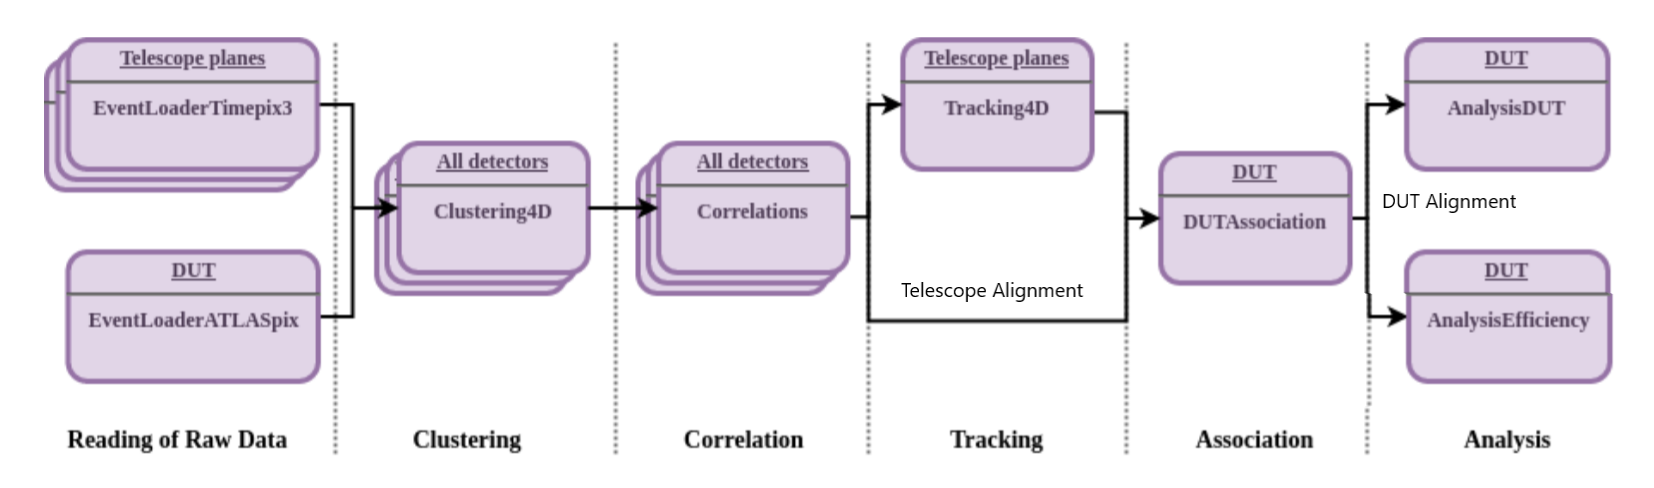
\includegraphics[height=0.3\textwidth]{images/corry.png}
  \caption{Overall track reconstruction chain with the standard clustering and tracking module. \cite{corry_track_reco}.}
  \label{fig:corry_track_reco}
\end{figure}

\chapter{Comparison of EUTelescope and Corryvreckan}\label{make}
Before using Corryvreckan to reconstruct particles for proton computed tomography, it is necessary to ensure that it's functioning properly
and is able to deliver equally valid results as the EUTelescope framework.
The chosen data sample is batch 3 of a DESY testbeam run from june 2020. Besides the six Mimosa26 sensors it contains two RD53a sensors
as DUT's in between the triplets and a FEI4 sensor as a time reference behind the telescope. The RD53a sensors are pixel sensors
manufactured in a $\SI{65}{\nano\meter}$ CMOS technology with a matrix of (400 $\times$ 192) \textmu m$^2$ pixels of
(50 $\times$ 50) \textmu m$^2$ size. Electrons with an energy of $\SI{5}{\GeV}$ were used to irradiate the sensors.
To compare the two software, the results of each individual
reconstruction step are analysed. \\

\section{Clustering}
After converting the hit information to their respective formats, the clustering is the first step performed by Corryvreckan and EUTelescope
to be investigated.
%It should be noted that no cut on the firing frequency is applied in any of the software in order to properly investigate their similarity, as the cut on the frequency in both frameworks is not defined similarly.
In figure \ref{fig:cluster_size} the determined cluster sizes of Corryvreckan and EUTelescope are shown for the second plane exemplary.
For both software, the charge-weighted center-of-gravity algorithm is used.

\begin{figure}
  %\centering
  \hspace{-2.5cm}
  \begin{subfigure}{0.62\textwidth}
      %\centering
      \includegraphics[height=0.82\textwidth]{plots/june_clustersize_tel1_corry.pdf}
  \end{subfigure}
  \begin{subfigure}{0.62\textwidth}
      %\centering
      %\hspace{0.9cm}
      \includegraphics[height=0.82\textwidth]{plots/june_clustersize_tel1_EU.pdf}
  \end{subfigure}
  \caption{Number of clusters of different sizes calculated by Corryvreckan shown on the left and for EUTelescope shown on the right.}
  \label{fig:cluster_size}
\end{figure}

The number of identified clusters is identical and the distribution looks similar implying an identical clustering process
and no differences due to the data conversion step. A closer look at the individual bin entries, shown in table \ref{tab:cluster_sizes} in the appendix,
confirms that the distributions are identical.

\section{Track reconstruction}
The alignment and final track reconstruction of Corryvreckan and EUTelescope are based on different algorithms, thus the
results will not be identical. However, their precision can still be compared based on the calculated residuals for each sensor.
Since they describe the distance between a cluster center and the corresponding interpolated track, the position of
residuals in global coordinates is an indicator of how well the alignment process worked. The standard deviation of a
residual curve reflects the spatial resolution $\sigma$ of a sensor, making the form of the residual another crucial indicator
for successful track reconstruction. Here, the spatial resolution is defined as ${\sigma = p/\sqrt{12}}$ with $p$ being the
pixel pitch of the sensor.

Figure \ref{fig:residualX} depicts the residuals of the second plane in x-direction calculated by both frameworks. Three iterations
of the alignment step have been performed and the tracks are reconstructed with a general broken lines algorithm in both software.

\begin{figure}
  %\centering
  \hspace{-2.5cm}
  \begin{subfigure}{0.62\textwidth}
      %\centering
      \includegraphics[height=0.82\textwidth]{plots/june_residualX_tel1_corry.pdf}
  \end{subfigure}
  \begin{subfigure}{0.62\textwidth}
      %\centering
      \hspace{0.95cm}
      \includegraphics[height=0.82\textwidth]{plots/june_residualX_tel1_EU.pdf}
  \end{subfigure}
  \caption{Residual in x-direction of the second sensor plane calculated by Corryvreckan on the left and EUTelescope on the right.}
  \label{fig:residualX}
\end{figure}

Both residuals are narrow and symmetric around their mean, which is smaller than $\SI{1}{\micro\meter}$ indicating a successful
alignment. The standard deviation of the residuals is smaller than the spatial resolution of the Mimosa26 sensor, being
$\sigma_{\text{M26}} = \SI{18.4}{\micro\meter}/\sqrt{12} \approx \SI{5.311}{\micro\meter}$ in both directions. This is possible due to
the center-of-gravity algorithm used for calculating the cluster center. While the arithmetic mean of the pixel centers can
only be as accurate as the spatial resolution of the pixels, weighting the amount of deposited charge in each pixel increases the
spatial resolution of the particle hit position for clusters with more than one pixel. Since the number of clusters with more than
one pixel is non-negligible, shown in figure \ref{fig:cluster_size}, the standard deviation of the residuals is expected to be
smaller than the sensor's spatial resolution, further indicating a valid track reconstruction for both frameworks.

\section{DUT residuals}
After the final track reconstruction with the telescope, the hit information on the DUT planes is compared to the
reconstructed tracks. Again, three iterations of alignment are performed for the DUT planes. In figure \ref{fig:residual_dut}, the residuals in the
x- and y-direction are shown for the FEI4 sensor.

\begin{figure}
  %\centering
  \hspace{-2.5cm}
  \begin{subfigure}{0.62\textwidth}
      %\centering
      \includegraphics[height=0.82\textwidth]{plots/june_residualX_dut2_corry.pdf}
  \end{subfigure}
  \begin{subfigure}{0.62\textwidth}
      %\centering
      \hspace{0.95cm}
      \includegraphics[height=0.82\textwidth]{plots/june_residualX_dut2_EU.pdf}
  \end{subfigure}
  \begin{subfigure}{0.62\textwidth}
    \hspace{-2.5cm}
      %\centering
      \includegraphics[height=0.82\textwidth]{plots/june_residualY_dut2_corry.pdf}
  \end{subfigure}
  \begin{subfigure}{0.62\textwidth}
    \hspace{-2.5cm}
      %\centering
      \hspace{0.95cm}
      \includegraphics[height=0.82\textwidth]{plots/june_residualY_dut2_EU.pdf}
  \end{subfigure}
  \caption{Residuals of the FEI4 sensor in x-direction in upper row and y-direction in the lower row. The plots on the left
  were created with Corryvreckan and the plots on the right with EUTelescope.}
  \label{fig:residual_dut}
\end{figure}

For both directions the residuals calculated by Corryvreckan and EUTelescope are similar. All mean values are below $\SI{1}{\micro\meter}$
indicating a successful alignment. The spatial resolution of the sensor in the horizontal and vertical direction is:
\begin{align*}
  &\sigma_{\text{FEI4},\text{x}} = \SI{50}{\micro\meter}/\sqrt{12} \approx \SI{14.434}{\micro\meter} \\
  &\sigma_{\text{FEI4},\text{y}} = \SI{250}{\micro\meter}/\sqrt{12} \approx \SI{72.169}{\micro\meter}
\end{align*}

Both software determined similar standard deviations, with the ones for the residuals in the vertical direction being close to
the corresponding spatial resolution of the sensor and the ones for the horizontal residuals being larger.

%In this batch only a third
%of the RD53a sensor volume has been depleted limiting the statistics and thus the alignment performance, which is based on
%the reconstructed tracks.

Results produced by the Corryvreckan framework showed noticeable similarities to the EUTelescope calculations. While the track
fitting process isn't identical, the quality of the reconstructed tracks determined by Corryvreckan is on par with EUTelescope.
